\chapter{Thiết kế cơ sở dữ liệu với MongoDB}

\section{Index trong MongoDB}
\subsection{Index là gì?}
Trong cơ sở dữ liệu, ta đã biết Index(chỉ mục) là một file cấu trúc lưu trữ trên ổ cứng tương ứng với một table hoặc một view nào đó trong cơ sở dữ liệu nhằm mục đích cải thiện tốc độ truy xuất dữ liệu từ table hoặc view đó.\\
Ở mục này, chúng ta sẽ tìm hiểu cách đánh index cũng như các loại index có trong MongoDB.
\subsection{Các loại index}

\subsubsection{Compound index (Chỉ mục hỗn hợp các khóa)}
Đây là chỉ mục được đánh trên nhiều trường khác nhau trong database. Loại index nay hữu ích khi chúng ta thực hiện câu truy vấn trên đòi hỏi nhiều trường trên dữ liệu. Ví dụ câu lệnh sau đây giúp tạo chỉ mục hỗn hợp các khóa trên MongoDB.\\
\begin{figure}[h!]
		\centering
		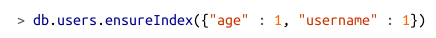
\includegraphics[scale=0.8]{charts/cpindex1.png}
		\caption{Câu lệnh tạo index hỗn hợp các khóa}
		\label{fig:cpindex}
\end{figure}
Trong câu lệnh trên, ta giả sử có một thư mục data có nhiều trường trong đó có trường username và age. Câu lệnh trên sẽ tạo ra chỉ mục đánh trên hai trường username và age đó. Số ứng với mỗi khóa trong câu lệnh chỉ mục trên thể hiện hướng của dữ liệu trên trường đó được sắp xếp như thế nào, với 1 là tăng dần, -1 là giảm dần. Trong ví dụ này thì age và username đều được đánh chỉ mục tăng dần.\\
Nếu ta có một tập dữ liệu gồm mà mỗi document trong dữ liệu đó bao gồm username có các giá trị như \textit{user01, user02, user03...} và age bao gồm các giá trị nguyên như \textit{1, 2, 3, 4...}. Thì chỉ mục sẽ có hình dạng như thế này
\pagebreak 
\begin{figure}[h!]
		\centering
		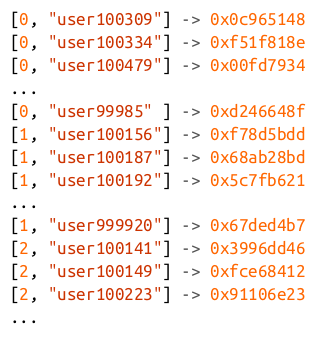
\includegraphics[scale=0.5]{charts/result.png}
		\caption{Kết quả}
		\label{fig:result}
\end{figure}
Mỗi index entry sẽ chứa lần lượt các giá trị của các trường là age ứng với giá trị nguyên và trường username ứng với các username \textit{user1, user2,...}. Và trong file index ấy do câu lệnh tạo index phía trên với trường age đứng trước tiên nên các entry được xếp tăng dần theo trường age và tiếp đến là tăng dần theo trường username có nghĩa là trước tiên chúng sắp xếp tăng dần theo trường age là số tuổi, tiếp đó với các user có cùng số tuổi thì sẽ sắp xếp tăng dần theo username. Bên cạnh đó, mỗi entry còn trỏ đến địa chỉ \textit{(được biểu diễn bằng chuỗi Hex)} của document được lưu trên đĩa.

\subsubsection{Unique index (Chỉ mục duy nhất)}
Với các hệ cơ sở dữ liệu như oracle, mySQL,... ta có primary index là dạng index đối với các trường có các giá trị không trùng nhau(unique). Với mongoDB, ta có Unique index hay còn gọi là chỉ mục duy nhất, các trường được đánh index này không được trùng nhau. Trong collection của mongoDB, trường "id" sẽ được tự động đánh là unique index.
\begin{itemize}
	\item \textbf{Compound unique index: }đây là sự kết hợp chỉ mục duy nhất với chỉ mục hỗn hợp các khóa. Cụ thể là, nếu có hai trường như name và address được đánh compound unique index thì một trong hai trường có thể có giá trị trùng nhau giữa các document nhưng không có document nào mà giống nhau ở cả hai trường đã được đánh index.
	\item \textbf{Các giá trị null: }trong quá trình insert dữ liệu, nếu một trường không có giá trị nào khi insert thi mongoDB sẽ mặc định giá trị đó là null. Nhưng nếu trường nói trên được đánh chỉ mục duy nhất thì nếu có thêm một trường bị gán giá trị null thì sẽ báo lỗi insert do trùng giá trị null.
\end{itemize}
\subsubsection{Sparse index (Chỉ mục thưa)}
Ở phần trên đề cập đến việc những trường được đánh chỉ mục duy nhất nhưng lại xuất hiện giá trị null. Trong những trường hợp có một trường nào đó trong collection mà có hoặc không cần insert giá trị nhưng bắt buộc trường đó là unique thì khi đó ta tạo chỉ mục duy nhất kết hợp với option sparse(thưa).\\
Ví dụ dưới đây là câu lệnh thực hiện việc tạo ra chỉ mục duy nhất trên trường email mà trường này không nhất thiết phải có giá trị. Các giá trị cấu hình cho unique và sparse lần lượt là "1" và "true":
\begin{figure}[h!]
		\centering
		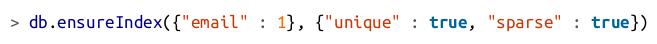
\includegraphics[scale=0.5]{charts/sparse.png}
		\caption{tạo chỉ mục duy nhất kết hợp với option sparse}
		\label{fig:spindex}
\end{figure}

\section{Các phép toán}
Sau khi data đã được lưu và thực hiện tạo index cần thiết trên mongoDB, trong công việc chúng ta có thể cần thực hiện nhiều tác vụ như phân tích theo nhiều cách khác nhau. Chính bì vậy mà mongoDB đã cung cấp một số công cụ để thực hiện các việc đó.\\
\subsection{Aggregation framework}
Aggragation có thể hiểu là sự tập hợp. Các Aggregation operation xử lý các bản dữ liệu và trả về kết quả đã được tính toán thành công. Các phép toán Aggregation nhóm các giá trị từ nhiều Document lại với nhau sau đó thực hiện nhiều phép toán đa dạng khác để trả về một kết quả duy nhất. Nói tới đây chúng ta liên tưởng tới phép toán count() và GROUPBY trong các hệ cơ sở dữ liệu SQL, các phép toán này tương ứng với Aggregation trong mongoDB.\\
Với Aggregation, mongoDB có hỗ trợ việc sử dụng thực hiện pipeline, có nghĩa là cho phép tạo ra một hoạt động hay tiên trình trên một số input và sử dụng output đó trở thành input cho các lệnh tiếp theo. Có một tập hợp các trạng thái có thể có, mỗi giai đoạn trên lấy một tập các document và tạo kết quả mà kết quả này được sử dụng cho các giai đoạn tiếp theo.
\textbf{Các giai đoạn trong Aggregation:}
\begin{itemize}
	\item \$match: công dụng như câu lệnh where trong các hệ cơ sở dữ liệu thông thường. Nó là hoạt động lọc giúp giảm số lượng document.
	\item \$project: giúp chọn một số trường cụ thể trong collection.
	\item \$group: thực hiện tập hợp lại các bản dữ liệu như phần đầu mục đã trình bày.
	\item \$sort: sắp xếp các document
	\item \$limit: giới hạn số document
	\item \$skip: Bỏ qua hay nhảy qua số document đã cung cấp.
	\item \$unwind: chia một document thành nhiều document. Tạo ra một số lượng document cho các giai đoạn khác nhau.
\subsection{MapReduce}	
\end{itemize}
